\documentclass{article}
\usepackage[polish]{babel}
\usepackage[T1]{fontenc}
\usepackage[utf8]{inputenc}
\usepackage{graphicx}
\usepackage{float}
\usepackage[bottom=1cm, right=1cm, left=1cm, top=1.5cm]{geometry}
\graphicspath{{../pliki}}



\title{%
  Cyberbezpieczeństwo - laboratoria 6 \\
  \large Jednokierunkowe funkcje skrótu \\ Algorytmy wymiany klucza
  }
\author{Patryk Łuszczek 272707}
\date{\today}
\begin{document}
\maketitle
\newpage
\tableofcontents
\newpage

\section{Jednokierunkowe funkcje skrótu}
3 stale dlugosci np. 20, 40, 60
porownac 3 funkcje dla tych dlosci bitow - sprawdzic czas
Do przeprowadzenia ataków zostały wykorzystane 2 pliki tekstowe w wersjach: oryginalna oraz sfałszowana.
\begin{enumerate}
  \item Plik 1
        \begin{enumerate}
          \item \textbf{Oryginalny: } Funkcja haszująca jest ważnym elementem techniki uwierzytelniania wiadomości.
                Otrzymuje ona dane wejściowe o różnej wielkości i wytwarza wartość skrótu o stałej
                wielkości.
                Funkcja haszująca używa funkcji kompresji w sposób powtarzalny, aby
                wygenerować n-bitową wartość wyjściową.
          \item \textbf{Fałszywy: } Funkcja haszująca jest ważnym elementem techniki uwierzytelniania wiadomości.
                Nie otrzymuje ona danych wejściowych o losowej wielkości i wytwarza wartość skrótu o stałej wielkości.
                Funkcja haszująca używa funkcji sinusoidalnej w celu zahaszowania, pliku.
        \end{enumerate}
  \item Plik 2
        \begin{enumerate}
          \item \textbf{Oryginalny: } A hash function is any function that can be used to map data of arbitrary size to fixed-size values, though there are some hash functions that support variable-length output.
                The values returned by a hash function are called hash values, hash codes, hash digests
          \item \textbf{Fałszywy: } A hash function is any function that is not used anymore, though there are some hash functions that may be still viable.
                The values returned by a hash function are used in the medical field to help patients with dementia.
        \end{enumerate}
\end{enumerate}

\subsection{Zadanie}
W celu wykonania zadania wybrano funkcję skrótu SHA-1. Zostały wczytane pliki tekstowe, oryginalny oraz fałszywy. Następnie przeprowadzono atak na z ustaloną długością bitów na 20.
Atak polegał na znalezieniu kolizji dla pierwszych 20-bitów hashu. Oba ataki zostały przeprowadzone pomyślnie.
\begin{table}[H]
  \centering
  \begin{tabular}{|c|c|c|}
    \hline
    \textbf{Plik / hash} & \textbf{oryginał}                                 & \textbf{fałszywy}                                 \\ \hline
    \textbf{Plik 1}      & \textbf{07AEA}044BFCF0EF704D3B150F8FE18F847ECDAF2 & \textbf{07AEA}B227C896E25C1AFB52B4ED431A580F13684 \\ \hline
    \textbf{Plik 2}      & \textbf{A983F}32783100C33E11664A8AF770AF08264BAB1 & \textbf{A983F}FE031226F03AD0289F79FA96EA4FC06CF5D \\ \hline
  \end{tabular}
\end{table}
Jak można zauważyć, pierwsz 20 bitów (czyli 5 znaków) hashu są identyczne. W przypadku pierwszego pliku, do obu wersji zostało dopisane 20 pustych znaków, dla drugiego pliku było to 10 i 7 znaków.


\subsection{Zadanie}
W tym zadaniu zostały wykorzystane następujące funkcje skrótu: MD5, SHA-1, RIPEMD-160, oraz następujące wartości długości bitów: 20, 40, 60

\begin{table}[H]
  \caption{Czas ataku dla różnych algorytmów i długości bitów}
  \centering
  \begin{tabular}{|c|c|c|c|c|}
    \hline
    \textbf{Algorytm / bity} & \textbf{20} & \textbf{40} & \textbf{60} & \textbf{80} \\ \hline
    \textbf{MD5}             & 0.01s       & 17s         & 1h          & 55 dni      \\ \hline
    \textbf{SHA-1}           & 0.02s       & 27s         & 53m         & 66dni       \\ \hline
    \textbf{RIPEMD-160}      & 0.03s       & 34s         & 2h 25m      & 180dni      \\ \hline
  \end{tabular}
\end{table}

\subsection{Jak rośnie czas realizacji ataku wraz ze wzrostem wartości parametru opisującego długość ustalonego ciągu bitów?}
Czas rezlizacji ataku jest ściśle powiązany z parametrem opisującym długość ciągu bitów. Wraz ze wzrostem tego parametru,
czas realizacji wzrasta wykładniczo. Dla długości 20bitów atak został przeprowadzony natychnmiastowo, natomiast dla długości 80 bitową, przewidywany czas realizacji wynosi kilkadziesiąt dni.
\subsection{Czy wybór funkcji skrótu ma wpływ na czas realizacji zadania poszukiwania kolizji?}
Jak można zauważyć na tabeli powyżej, czas realizacji ataku jest zależny od funkcji skóru. Najdłuższe czasy realizacji
zostały zanotowan dla funkcji RIPEMD-160, natomiast najkrótsze dla funkcji MD5, oprócz eksperymentu dla 60 bitów, gdzie SHA-1 okazało się szybsze.
% te nastepne do wlasnego zastanowienia/ wyszukania
\subsection{Na czym polega przewaga modyfikowania dwóch dokumentów nad poszukiwaniem kolizji przy modyfikacji tylko jendego dokumentu?}
Kiedy modyfikowane są oba dokumenty, rośnie przestrzeń poszukiwań kolizji, co znacznie ułatwia jej znalezienie.
\subsection{Czy w świetle uzyskanych wyników możemy ufać funkcjom skrótu?}
Mimo, że eksperyment został przeprowadzony tylko dla 60 bitów, można stwierdzić, że funkcje skrótu mają swoje słabości i ograniczenia. Dla wartości bitów podanych w eksperymencie
udało się znaleźć kolizję, co wskazuje na to, że przepadane funkcje skrótu nie śa idealne. Dodatkowo funkcje takie jak MD5 oraz SHA-1 obecnie są uważane za niebezpiecznie i nie są zalecane.
Więc w celu zwiększenia bezpieczeńswa, zaleca się korzystanie z silniejszych funkcji, takichj jak np. SHA-256 lub SHA-3.
\subsection{Jakiego typu problemy zostały zidentyfikowane dla popularnych funkcji skrótu (MD5, SHA)?}
W przypadku obu tych funkcji, zostało udowodnione, że śa ole podatne na kolizje, i że nie powinny być używane
do zastosowań kryptograficznych (podpisy cyfrowe, certyfikaty, itp.). Dla MD5, zostało to pokazane już w 2004 roku. W przypadku SHA-1, w 2017 roku został
zaprezentowany pierwszy publiczny atak kolizji nazwany "SHAttered". Zostały pokazane dwa całkiem niepodobne pliki PDF, a sam atak miał być 100 000 razy szybszy
niż atak brute-force z wykorzystaniem ataku urodzinowego.

\section{Wymiana klucza kryptograficznego}
tutaj screeny z podpisem ktory to klient

\begin{itemize}
  \item Generowanie wspólnego klucza DH:
        \begin{figure}[H]
          \centering
          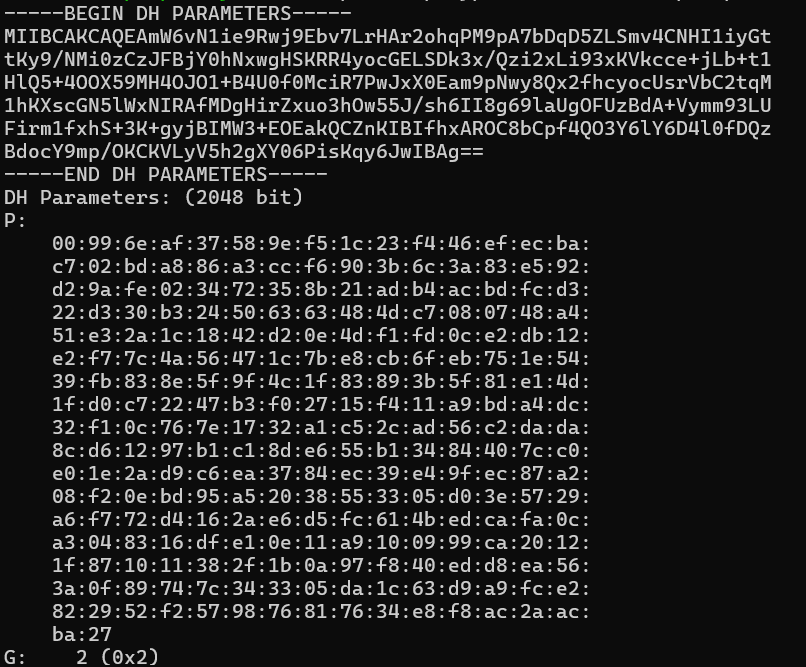
\includegraphics[width=0.5\textwidth]{klucz_wspolny.png}
        \end{figure}
  \item  Klucz dla klienta 1:
        \begin{figure}[H]
          \centering
          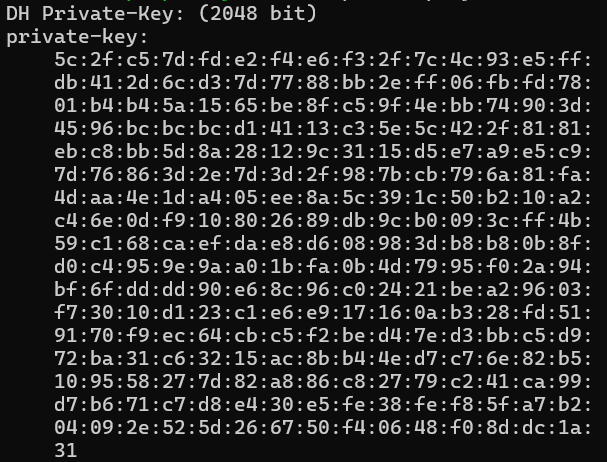
\includegraphics[width=0.5\textwidth]{client1_private_key.png}
        \end{figure}
  \item Klucz dla klienta 2:
        \begin{figure}[H]
          \centering
          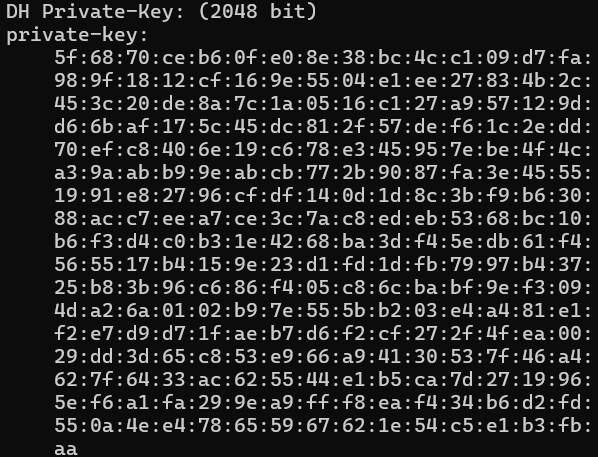
\includegraphics[width=0.5\textwidth]{client2_private_key.png}
        \end{figure}
  \item Klucz tajny dla obu klientów jest jednakowy, komenda cmp nie zwróciła żadnego wyniku, który wskazywałby na różnice między nimi
  \item Secret key 1
        \begin{figure}[H]
          \centering
          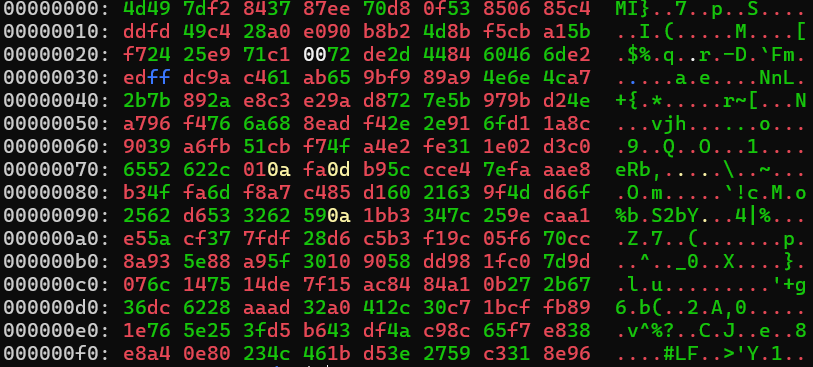
\includegraphics[width=0.5\textwidth]{secret_key1.png}
        \end{figure}
  \item Secret key 2
        \begin{figure}[H]
          \centering
          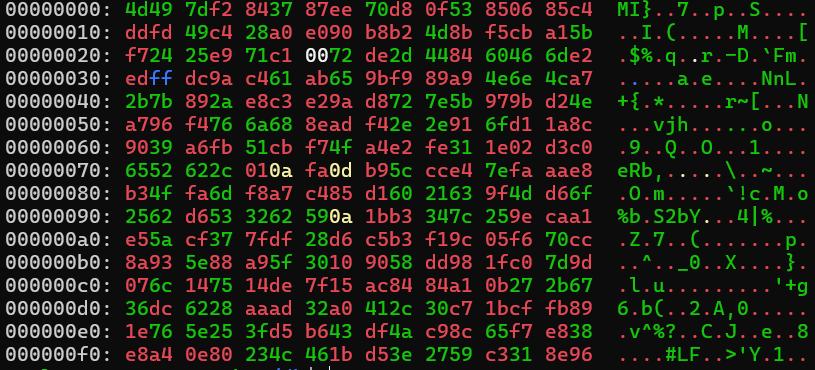
\includegraphics[width=0.5\textwidth]{secret_key2.png}
        \end{figure}
\end{itemize}

\subsection{Który sposób wymiany kluczy gwarantuje większe bezpieczeństwo i dlaczego (RSA vs DH)}
\subsection{Jakie jest ryzyko dla podmiotów korzystających z protokołu wymiany kluczy DH?}
Jednym z zasadnicych zagrożen wynikających z protokołu wymiany kluczy DH jest podatność na atak typu Man-In-The-Middle. Wiąże się to z brakiem
mechanizmu autoryzacji, który pozwalałbym na weryfikację wiadomości otrzymanych od drugiej strony. Atakujący może dowolnie manipulować wiadomościami bez wiedzy żadnej ze stron.
Podczas takiego ataku, atakujący może uzyskać dostęp do do wiadomości, poprzez zmianę transmitowanego klucza na własny. W celu zabezbieczenia się przed tego typu atakiem,
zaleca się wykorzystanie pewnej formy uwierzytelnienia, np. protokołu PAKE (Password Authentification Key Agreement).
\subsection{Jakie są inne metody określania wspólnego klucza krypotgraficznego (oprócz DH)}
\subsection{Który element protokołu DH nie jest przesyłany między klientami? Jak to wpływa na kwestie bezpieczeństwa?}
W protokole DH nie jest przesyłany klucz prywatny, ustalany indywidualnie dla każdej ze stron. Dzięki kluczowi prywatnemu, strony mogą ustalić wspólny klucz, który jest obecnie niemożliwy do odszyfrowania,
jeśli poszczególne parametry są wystarczająco skomplikowane.
\subsection{Sprawdź czy w ostatnim punkcie udał się ustalić ten sam klucz dla obu klientów. Uwzlgędnij w raporcie treść uzgodniionego tajnego klucza.}
W wyniku eksperymentu udało się uzyskać ten sam klucz dla obu klientów, jego treść została zamieszczona we wcześniejszej części raportu.
\end{document}